\documentclass[11pt, solution, letterpaper]{format}
\usepackage[utf8]{inputenc}
\setlength{\parindent}{0 in}

\usepackage{tikz}
\usetikzlibrary{arrows,automata}
\usepackage{amsmath}
\usepackage{graphicx}
\graphicspath{ {./images/} }
\usepackage[utf8]{inputenc}
\usepackage{enumerate}
\usepackage{amsmath,amssymb,amsthm}
\usepackage{listings}
\renewcommand{\qedsymbol}{$\blacksquare$}
\setlength\parindent{0pt}
\usepackage{tikz}
\usepackage{pgf}
\usepackage{tikz}
\usetikzlibrary{arrows,automata}
\usepackage{hyperref}
\newcommand{\noin}{\noindent}
\usepackage{enumerate}
\usepackage{tikz}
\usepackage{pgf}
\usepackage{tikz}
\usepackage{hyperref}
% \usepackage{booktabs}
\usepackage{cancel}

% \pagestyle{empty}

\setlength{\oddsidemargin}{-0.25 in}
\setlength{\evensidemargin}{-0.25 in}
\setlength{\topmargin}{-0.9 in}
\setlength{\textwidth}{7.0 in}
\setlength{\textheight}{9.0 in}
\setlength{\headsep}{0.75 in}
\setlength{\parindent}{0 in}
% \setlength{\parskip}{-.10 in}
\usepackage{epsf}
\usepackage{pseudocode}
% \usepackage{times}
% \usepackage{mathptm}

\def\O{\mathop{\smash{O}}\nolimits}
\def\o{\mathop{\smash{o}}\nolimits}
\newcommand{\e}{{\rm e}}
\newcommand{\R}{{\bf R}}
\newcommand{\Z}{{\bf Z}}
\newcommand\tab[1][1cm]{\hspace*{#1}}




\begin{document}
Problem Set 7\\
Julia Pearl\\

I collaborated with Rodrigo Daboin Sanchez and Noah Epstein. All code and problems were done independently.
\clearpage
\section{Recurrence}
Suppose we are given a maximum flow in a graph G = (V,E) with source s, sink t, and integer capacities.
(That is, we’re given both the maximum flow value, as well as the amount of flow that goes along each edge
to achieve that value.) Now the capacity of a given edge e is increased by 1. Give a linear time O(V+E)
algorithm for computing the new maximum flow. Similarly, give a linear time O(V + E) algorithm for
computing the new maximum flow if the capacity of a given edge e is decreased by 1.\\

\textbf{Increasing an Edge Capacity}\\

\textbf{Defining Variables}\\
Let us define variables for this problem. 
\begin{itemize}
    \item We have a graph G. 
    \item G has a max flow of $F$.
    \itme G's edge $(u, v)$  has a capacity $C(u, v)$ and a flow of $f(u, v)$. 
    \item In $G'$, $(u, v)$'s capacity is equal to $C(u, v) + 1 = C'(u, v)$. In $G'$, $(u, v)$'s flow is $f'(u, v)$.
    \item Once we update the graph so that $(u, v)$ has a capacity $C'(u, v)$, we will refer to the graph as $G'$ with a max flow of $F'$.
\end{itemize}  

\textbf{Obtaining $F'$}\\
We will go through the steps of a linear time algorithm that will obtain $F'$. \\

\textbf{Range of $F'$}\\
However, before we go through the steps of the algorithm, we will clarify the potential range of $F'$. Because we are updating the capacity of only one edge by one, $F'$ can only be equal to $F$ or $F$ + 1. We identify two cases of this problem. One in which, $(u, v)$ at some point in obtaining $F$ from $G$ acts as a bottleneck to a path or it does not. \\

The first case: If $(u, v)$ were to never act as a bottleneck for any path while yielding $F$ from $G$, then updating the capacity of $(u, v)$ by 1 would have no effect on the $F'$. In this case, the residual network after passing $F$ through G yields $(u, v)$ with a remnant (positive integer) forward capacity that is not utilized and is restrained by other edge capacities. That remnant (positive integer) capacity would be increased by 1. In this case, $F$ = $F'$. In the algorithm, we will check for this case in our first step by checking if the $f(u, v) < C(u, v)$.  \\

The second case: If $(u, v)$ were to act as a bottleneck at some point for a path from $F$ to $G$, then increasing its capacity by 1 can only, at most, increase $F$ by 1.  \\
There are two subcases in which $(u, v)$ acts as a bottleneck that would yield different effects on $F'$. 
Subcase A: when $(u, v)$ acts as a bottleneck, if there exists another edge with the same forward moving capacity as $(u, v)$ also acting as a bottleneck (for a path) at that point in the residual network, then increasing $(u, v)$'s capacity would have no effect on the total flow because $G'$ has other limitations. $F'$ would equal $F$.\\
Subcase B: If $(u, v)$ were to be the singular bottleneck to a path in the final point of the residual network, then increasing $(u, v)$'s capacity by one would only allow 1 more unit of flow to be passed. $F'$ would equal $F$ + 1.

This means that the maximum value for $F'$ that we could potentially find (and the only value that we need to search for) is equal to $F$ + 1. \\

\textbf{The Algorithm to yield $F'$}
\begin{enumerate}
\item First, we pass $F$ through $G$, also constructing $G$'s residual network.***\\
***I don't know if we initially know $f(u, v)$ or if we need to pass $F$ through $G$ to know $f(u, v)$. If we already know f(u, v), then if $f(u, v) < C(u, v)$ we can return $F$, yielding that $F'$ is equal to $F$.
\item Then, we check if $f(u, v) < C(u, v)$. 
\begin{enumerate}
\item If true, then (u, v) is not a bottleneck for any path in G, and updating its capacity by 1 will have no effect on the $F'$. This is because of the first case explained previously. Thus, we can return $F$, yielding that $F'$ is equal to $F$.
\end{enumerate}
\item (Else): We update the capacity of (u, v) to equal $C'(u, v)$, equivically updating $G$ to $G'$.
\item We run Ford-Fulkerson with DFS--searching for an augmented path in $G'$. Because DFS has a runtime dependent upon max flow, it's good to note that here, we are at most passing one unit of flow through this $G'$, so the max flow has an upper bound of 1.
\begin{enumerate}
\item If we successfully passed one more unit of flow across $G'$, then we can return $F$ + 1, yielding that $F'$ is equal to $F$ + 1.
\item If we did not pass any more units of flow across $G'$, then we can return $F$, yielding that $F'$ is equal to $F$.
\end{enumerate}
\end{enumerate}

In this algorithm, we have yielded $F'$. Examining at this algorithm for runtime, constructing the residual network of a graph takes O(E) time because we are given both integer capacities of the edges and the amount of flow that goes along each edge to achieve the max flow. Checking the flow afterwards takes O(1) time. Running Ford-Fulkerson DFS with a max flow of 1 yields O(E1*) or O(E) time. It's linear!\\

\textbf{Decreasing an Edge Capacity}\\

\textbf{Defining Variables}\\
Let us define variables for this problem. 
\begin{itemize}
    \item We have a graph G. 
    \item G has a max flow of $F$.
    \itme G's edge $(u, v)$  has a capacity $C(u, v)$ and a flow of $f(u, v)$. 
    \item In $G'$, $(u, v)$'s capacity is equal to $C(u, v) - 1 = C'(u, v)$. In $G'$, $(u, v)$'s flow is $f'(u, v)$.
    \item Once we update the graph so that $(u, v)$ has a capacity $C'(u, v)$, we will refer to the graph as $G'$ with a max flow of $F'$.
\end{itemize}  

\textbf{Obtaining $F'$}\\
We will go through the steps of a linear time algorithm that will obtain $F'$. \\

\textbf{Range of $F'$}\\
However, before we go through the steps of the algorithm, we will clarify the potential range of $F'$. Because we are updating the capacity of only one edge by one, $F'$ can only be equal to $F$ or $F$ - 1. We identify two cases of this problem. One in which, $(u, v)$ at some point in obtaining $F$ from $G$ acts as a bottleneck to a path or it does not. \\

The first case: If $(u, v)$ were to never act as a bottleneck for any path while yielding $F$ from $G$, then updating the capacity of $(u, v)$ by 1 would have no effect on the $F'$. In this case, the residual network after passing $F$ through G yields $(u, v)$ with a remnant (positive integer) forward capacity that is not utilized and is restrained by other edge capacities. That remnant (positive integer) capacity would be decreased by 1. In this case, $F$ = $F'$. In the algorithm, we will check for this case in our first step by checking if the $f(u, v) < C(u, v)$.  \\

The second case: If $(u, v)$ were to act as a bottleneck at some point for a path from $F$ to $G$, then decreasing its capacity by 1 can only, at most, decrease $F$ by 1. $F'$ would equal $F$ - 1.\\

% This means that the minimum value for $F'$ that we could potentially find (and the only value that we need to search for) is equal to $F$ - 1. \\

\textbf{The Algorithm to yield $F'$}
\begin{enumerate}
\item First, we pass $F$ through $G$, also constructing $G$'s residual network.***\\
***I don't know if we initially know $f(u, v)$ or if we need to pass $F$ through $G$ to know $f(u, v)$. If we already know f(u, v), then if $f(u, v) < C(u, v)$ we can return $F$, yielding that $F'$ is equal to $F$.
\item Then, we check if $f(u, v) < C(u, v)$. 
\begin{enumerate}
\item If true, then (u, v) is not a bottleneck for any path in G, and updating its capacity by 1 will have no effect on the $F'$. This is because of the first case explained previously. Thus, we can return $F$, yielding that $F'$ is equal to $F$.
\end{enumerate}
\item (Else): Define p1, a singular path from u to s.
\item: Define p2, a singular path from t to v.
\item: Pass one unit of flow through from p2 to (u, v) to through p1, updating $G$'s residual network. We have just changed G's max flow from $F$ to $F$ - 1. This is the lowest that the max flow could potentially be. 
\item: We update the capacity of (u, v) to equal $C'(u, v)$, equivically updating $G$ to $G'$.
\item We run Ford-Fulkerson with DFS--searching for an augmented path in $G'$. Because DFS has a runtime dependent upon max flow, it's good to note that here, we are at most passing one unit of flow through this $G'$, so the max flow has an upper bound of 1.
\begin{enumerate}
\item If we successfully passed one more unit of flow across $G'$, then we can return $F$, yielding that $F'$ is equal to $F$.
\item If we did not pass any more units of flow across $G'$, then we can return $F$ - 1, yielding that $F'$ is equal to $F$ - 1.
\end{enumerate}
\end{enumerate}

\textbf{Runtime}\\
In this algorithm, we have yielded $F'$. Examining at this algorithm for runtime, constructing the residual network of a graph takes O(E) because we are given both integer capacities of the edges and the amount of flow that goes along each edge to achieve the max flow.. Checking the flow afterwards takes O(1) time. Identifying p1 and p2 takes O(E) time because we are looking for one valid paths amidst all paths. Passing one unit of flow backwards on the graph takes O(E).  Running Ford-Fulkerson DFS with a max flow of 1 yields O(E1*) or O(E) time. It's linear!

\clearpage
\section{Max Flow}
If we restrict the problems we look at, sometimes hard problems like counting the number of independent sets
are in a graph become solvable. For instance, consider a graph that is a line on n vertices. (That is, the vertices
are labelled 1 to n, and there is an edge from 1 to 2, 2 to 3, etc.) How many independent sets are there on a
line graph? Also, how many independent sets are there on a cycle of n vertices? (Hint: In this case, we want
to express your answer in terms of a family of numbers – like “For n vertices the number of independent sets
is the nth prime.” And that’s not the answer.)
Similarly, describe how you could quickly compute the number of independent sets on a complete binary tree.
(Here, just explain how to compute this number.) Calculate the number of independent sets on a complete
binary tree with 127 nodes. (Warning: it’s a pretty big number.)\\

\textbf{A Line with N Vertices}\\
Let us call the number of independent sets on a line with n vertices equal to $L_n$. To find $L_n$, we construct a line with n vertices {$v_1, ... v_n$}: $$\pmb{v_1-v_2-  ...  -v_n}$$
In order to obtain value of $L_n$, we consider two values whose sum cover all of $L_n$: \textbf{N1)} the number of all of the independent sets on a line of n vertices that \textbf{do not} include $v_n$ and \textbf{N2)} the number of all of the independent sets on a line of n vertices that \textbf{do} include $v_n$: $$L_n = N1 + N2$$
\textbf{N1)} Reiterating, N1 is the number of all of the independent sets that do not include $v_n$ on a line of n vertices. Because N1 only counts the independent sets \textbf{not} containing $v_n$, we can picture N1 as a line of n - 1 vertices:
$$\pmb{v_1-v_2-  ...  -v_{n-1}}(-v_n)$$
Thus, we can say that N1 is equal to the number of independent sets for the n-1th vertex. This number is equal to $L_{n-1}$. \\

\textbf{N2)} Reiterating, N2 is the number of all of the independent sets on a line of n vertices that \textbf{do} include $v_n$. Because the sets counted in N2 include $v_n$, by the definition of independent sets, we know that $v_{n-1}$ is not included in any of the sets making up N2. We can picture N2 as a line of independent sets with the nth vertex included, the n-1th vertex not included, and the line of n - 2 vertices:
$$\pmb{v_1-v_2-  ... }-v_{n-1}-\pmb{v_n}$$
We can say that N2, or the sum of independent sets for the nth vertex that do include $v_n$, is equal to the total sum of independent sets of vertex $v_{n-2}$, $L_{n-2}$. \\

Summing N1 and N2, 
$$L_n = L_{n - 1} + L_{n - 2}$$

\textbf{Base Cases}\\
Our base cases are: \\
\textbf{0 vertices}, in which there is only one independent set which is equal to the empty set: $L_0 = 1$.\\
And \textbf{1 vertex}, which which there are two independent sets present, the empty set and the set containing the single vertex: $L_1 = 2$.\\


After these two base cases,
$L_n = L_{n - 1} + L_{n - 2}$ holds.

Thus:
$$L_0 = 1$$$$L_1 = 2$$$$L_n = L_{nc - 1} + L_{n - 2} \text{ for n }> 1$$
Notably, this summation pattern is equal to the fibonacci series, with the base cases beginning at the 2nd fibonacci number.\\

\textbf{A Cycle with N Vertices}\\
Let us call the number of independent sets on a cycle with n vertices equal to $C_n$. To find $C_n$, we construct a cycle with n vertices {$v_1, ... v_n$}: $$\pmb{-v_1-v_2-  ...  -v_n-}$$
In order to obtain value of $C_n$, we consider two values whose sum cover all of $C_n$: \textbf{N1)} the number of all of the independent sets on a cycle of n vertices that \textbf{do not} include $v_n$ and \textbf{N2)} the number of all of the independent sets on a cycle of n vertices that \textbf{do} include $v_n$: $$C_n = N1 + N2$$
\textbf{N1)} Reiterating, N1 is the number of all of the independent sets that do not include $v_n$ on a cycle of n vertices. Because N1 only counts the independent sets \textbf{not} containing $v_n$, we can picture N1 as the following:
$$\pmb{-v_1-v_2-  ...  -v_{n-1}}-v_n-$$
With the nth vertex removed, the cycle becomes a line sizes n - 1. From part one of this problem, we know the sum of independent sets in a line including n-1 vertices. This is equal to $L_{n-1}$. \\

\textbf{N2)} Reiterating, N2 is the number of all of the independent sets on a cycle of n vertices that \textbf{do} include $v_n$. Because the sets counted in N2 include $v_n$, by the definition of independent sets, we know that $v_{n-1}$ and $v_1$ are not included in any of the sets making up N2. We can picture N2 as the following:
$$- v_1 - \pmb{-v_2-  ...  -v_{n-2}}-v_{n-1}-\pmb{v_n}-$$
With the n-1th vertex and the 1st vertex removed, the cycle becomes a line sizes n - 3 plus the nth vertex. From part one of this problem, we know the sum of independent sets in a line including n-3 vertices. This is equal to $L_{n-3}$. \\

Summing N1 and N2, 
$$C_n = L_{n - 1} + L_{n - 3}$$

\textbf{Base Cases}\\
Instead of building base cases for $C_n$, we can create an additional base case for $L_n$ and have a working $C_n$:
When n is less than one, $L_n$ = 1.
that for $L_n$, if n is 

Our base cases are: \\
\textbf{0 vertices}, in which there is only one independent set which is equal to the empty set: $C_0 = 1$.\\
And \textbf{1 vertex}, which which there are two independent sets present, the empty set and the set containing the single vertex: $C_1 = 2$.\\
And \textbf{2 vertices}, which which there are three independent sets present, the empty set, the set containing one of the two vertices, and the set containing the other of the two vertices: $C_2 = 3$.\\


After these two base cases,
$C_n = L_{n - 1} + L_{n - 3}$ holds.

Thus:
$$C_0 = 1$$$$C_1 = 2$$$$C_2 = 3$$$$C_n = L_{n - 1} + L_{n - 3} \text{ for n }> 2$$

\textbf{A Full, Complete Binary Tree with N Levels}\\
For the extent of this problem, a FCB tree will be equal to a full and complete binary tree).

Let us call the number of independent sets on a FCB tree with n levels equal to $B_n$. While the problem states that we need to calculate the number of sets for 127 nodes, a complete binary tree with 127 nodes is equal to FCB tree with 7 levels. So, we can just find how to calculate the number of independent sets based just on levels (n levels). To find this number, $B_n$, we construct a FCB tree with n levels:\\
\begin{center}
\begin{tikzpicture}[level distance=1.5cm,
  level 1/.style={sibling distance=3cm},
  level 2/.style={sibling distance=1.5cm}]
  \node {root: $\pmb{level_n}$}
    child {node {$\pmb{level_{n-1}}$}
      child {node {$\pmb{level_{n-2}}$}}
      child {node {$\pmb{level_{n-2}}$}}
    }
    child {node {$\pmb{level_{n-1}}$}
    child {node {$\pmb{level_{n-2}}$}}
      child {node {$\pmb{level_{n-2}}$}}
    };
\end{tikzpicture}\\
....................(etc).................................
\end{center}

\\

In order to obtain value of $B_n$, we consider two values whose sum cover all of $B_n$: \textbf{N1)} the number of all of the independent sets on a FCB tree of n levels that \textbf{do not} include the root $level_n$ and \textbf{N2)} the number of all of the independent sets on a FCB tree of n levels that \textbf{do} include $level_n$: $$B_n = N1 + N2$$
\textbf{N1)} Reiterating, N1 is the number of all of the independent sets that do not include $level_n$ on a FCB tree. Because N1 only counts the independent sets \textbf{not} containing $level_n$, we can picture N1 as 2 FCB trees of n-1 levels:
\begin{center}
\begin{tikzpicture}[level distance=1.5cm,
  level 1/.style={sibling distance=3cm},
  level 2/.style={sibling distance=1.5cm}]
  \node {$level_n$}
    child {node {root: $ \pmb{level_{n-1}}$}
      child {node {$\pmb{level_{n-2}}$}}
      child {node {$\pmb{level_{n-2}}$}}
    }
    child {node {root: $\pmb{level_{n-1}}$}
    child {node {$\pmb{level_{n-2}}$}}
      child {node {$\pmb{level_{n-2}}$}}
    };
\end{tikzpicture}\\
....................(etc).................................
\end{center}

Thus, we can say that N1 is equal to the combination of the left and the right independent sets for a FCB tree with n-1 levels. This number is equal to $B_{n-1}^2$. \\

\textbf{N2)} Reiterating, N2 is the number of all of the independent sets on a FCB tree with n levels that \textbf{do} include $level_n$. Because the sets counted in N2 include $level_n$, by the definition of independent sets, we know that all vertices of $level_{n-1}$ are not included in any of the sets making up N2. Because N1 only counts the independent sets \textbf{not} containing $level_{n-1}$, we can picture N1 as 2*2 so 4 FCB trees of n-2 levels with the nth level still included (from a distance):

\begin{center}
\begin{tikzpicture}[level distance=1.5cm,
  level 1/.style={sibling distance=7cm},
  level 2/.style={sibling distance=3cm}]
  \node {$\pmb{level_n}$}
    child {node {$level_{n-1}$}
      child {node {root: $\pmb{level_{n-2}}$}}
      child {node {root: $\pmb{level_{n-2}}$}}
    }
    child {node {$level_{n-1}$}
    child {node {root: $\pmb{level_{n-2}}$}}
      child {node {root: $\pmb{level_{n-2}}$}}
    };
\end{tikzpicture}\\
....................(etc).................................
\end{center}

We can say that N2 is equal to the combination of 4 independent sets for a FCB tree with n-2 levels. This number is equal to $B_{n-2}^4$. \\

Summing N1 and N2, 
$$B_n = B_{n - 1}^2 + B_{n - 2}^4$$

\textbf{Base Cases}\\
Our base cases are: \\
\textbf{0 levels}, in which the BCF tree is graphically equivalent to a line with 0 vertices: $B_0 = L_0 = 1$.\\
\textbf{1 level}, in which the BCF tree is graphically equivalent to a line with 1 vertex: $B_1 = L_1 = 2$.\\
And \textbf{2 levels}, in which the BCF tree is graphically equivalent to a line with 3 vertices: $B_2 = L_3 = 5$.\\


After these three base cases,
$B_n = B_{n - 1}^2 + B_{n - 2}^2$ holds.

Thus:
$$B_0 = 1$$$$B_1 = 2$$$$B_2 = 5$$$$B_n = B_n = B_{n - 1}^2 + B_{n - 2}^4 \text{ for n }> 2$$


For a binary tree with 127 nodes or 7 levels, there are 13345346031444632841427643906 independent sets.


\clearpage
\section{Max-k-Cut}
Consider the problem MAX-k-CUT, which is like the MAX CUT algorithm, except that we divide the vertices
into k disjoint sets, and we want to maximize the number of edges between sets. Explain how to generalize
both the randomized and the local search algorithms for MAX CUT to MAX-k-CUT and prove bounds on
their performance.\\

Before going into the randomized or the local search algorithms for Max Cut, it is important to note that because Max Cut divides vertices into 2 disjoint sets, Max Cut is equal to Max-k-Cut when k = 2. Thus, for the rest of this problem, let us refer to Max-Cut as Max-2-Cut.

\textbf{Randomized Search Algorithm} 
Let's initially focus on generalizing the randomized algorithm from Max-2-Cut Max-k-Cut. We will write out the steps to the randomized algorithm when k = 2, and then, go through and generalize the algorithm. 
\begin{enumerate}
  \item The randomized algorithm for Max-2-Cut begins by dividing the vertices into 2 sets.
  \item The vertices are placed into 1 of the 2 total sets with a probability of $\frac{1}{\text{number of sets}}=\frac{1}{2}$. 
  \item  Each edge is made up of two vertices. For each edge (u, v), the probability that it will cross the cut is equal to 1 minus the probability that the vertices belong to the same set. 
  \begin{enumerate}
  \item The probability that u belongs to the same set as u is 1. 
  \item The probability that v belongs to the same set as u is $\frac{1}{\text{number of sets}} = \frac{1}{2}$.
  \item  The probability that u and v belong to the same set is 1*$\frac{1}{2} = \frac{1}{2}$.
  \item 1 minus the probability that v and u belong to the same set is equal to 1 - $\frac{1}{2}$ = $\frac{1}{2}$.
  \end{enumerate}
  \item Restating the probability calculated by the previous step, the probability that each edge will cross the cut is equal to $\frac{1}{2}$
  \item The expected value of edges that will cross the cut is the total number edges times this probability, so  $\frac{1}{2}$ of the edges.
  \item    Since the most we could have is for all the edges to cross the cut, this random assignment will, on average, be within a factor of 2 of optimal.
\end{enumerate}

Let's rewrite these steps and sub k for 2:
\begin{enumerate}
  \item The randomized algorithm for Max-k-Cut begins by dividing the vertices into k sets.
  \item The vertices are placed into 1 of the k total sets with a probability of $\frac{1}{\text{number of sets}}=\frac{1}{k}$. 
  \item  Each edge is made up of two vertices. For each edge (u, v), the probability that it will cross the cut is equal to 1 minus the probability that the vertices belong to the same set. 
  \begin{enumerate}
  \item The probability that u belongs to the same set as u is 1. 
  \item The probability that v belongs to the same set as u is $\frac{1}{\text{number of sets}} = \frac{1}{k}$.
  \item  The probability that u and v belong to the same set is 1*$\frac{1}{k} = \frac{1}{k}$.
  \item 1 minus the probability that v and u belong to the same set is equal to 1 - $\frac{1}{k}$ = $\frac{k - 1}{k}$. 
  \end{enumerate}
  \item Restating the probability calculated by the previous step, the probability that each edge will cross the cut is equal to $\frac{k - 1}{k}$
  \item The expected value of edges that will cross the cut is the total number edges times this probability, so  $\frac{k - 1}{k}$ of the edges.
  \item    Since the most we could have is for all the edges to cross the cut, this random assignment will, on average, be within a factor of $\frac{k}{k - 1}$ of optimal.
\end{enumerate}

These are the steps for generalizing the randomized algorithm from Max-2-Cut to Max-k-Cut. As we have proved, the randomized algorithm for Max-k-Cut has a bound within  within a factor of $\frac{k}{k - 1}$ of optimal.\\

\textbf{Local Search Algorithm} \\
Now, let's focus on generalizing the local search algorithm from Max-2-Cut Max-k-Cut. We will write out the steps to the local search algorithm when k = 2, and in the following step, prove the bounds of this algorithm. Then, we will go through and generalize the algorithm as well as the bounds for any k. \\

\textbf{Steps to Local Search Algorithm Max-2-Cut} 
\begin{enumerate}
\item  We will split the vertices into 2 sets, S1 and S2.
\item  Start with all vertices arbitrarily at S1 (one side of the cut).
\item   Now, if you can
switch a vertex into a different set so that it increases the number of edges across the cut, do so. Repeat this action
until the cut can no longer be improved by this simple switch.
\item  We switch vertices at most 1*$|E|$ times (since each time, the number of edges across the cut increases). We will review the lecture's proof below that when the Local Search Algorithm for Max-2-Cut completes, we are within a factor of 2 of the optimal.
\end{enumerate}
\textbf{Proving Bounds of Local Search Algorithm Max-2-Cut} \\

Let us show that when the algorithm finishes we are within a factor of 2 of the optimal. Another way of stating this is that when the process finishes, at least |E|/2 edges lie in the cut. We can count the edges in the cut in the following way: \\
We have a running sum that represents our cut C. We start with one of our groups S1. For every vertex in S1, for each edge that vertex is connected to whose other vertex is not also in S1, we add 1/2 to C. We repeat this process for our remaining group, S2. We are adding 1/2 to our running sum because we know that we are counting each edge that crosses the cut twice (because of both of its vertices). \\  

Hence the cut C satisfies
$$C =\frac{1}{2} * (\sum_{v\in S1} |\{w: (v, w) \in E, w \in S2 \}| + \sum_{v\in S2} |\{w: (v, w) \in E, w \in S1 \}| )$$

Since we are using the local search algorithm, the number of edges that cross the cut must be equal to the probability of 2 vertices being in different sets. Thus, at least half the edges from any vertex v must lie in the set opposite
from v; otherwise, we could switch what side vertex v is on, and improve the cut. Hence, if vertex v has degree d(v),
then
$$C =\frac{1}{2} * (\sum_{v\in S1} |\{w: (v, w) \in E, w \in S2 \}| + \sum_{v\in S2} |\{w: (v, w) \in E, w \in S1 \}| )$$
$$\geq \frac{1}{2} * (\sum_{v\in S1} \frac{d(v)}{2} + \sum_{v\in S2} \frac{d(v)}{2})$$
$$=\frac{1}{4} * (\sum_{v\in V} d(v) $$ 
$$ = \frac{1}{2}*|E|$$
where the last equality follows from the fact that if we sum the degree of all vertices, we obtain twice the number of
edges, since we have counted each edge twice.

Now, we generalize the local search algorithm from Max-2-Cut Max-k-Cut. We will adjust the steps to the local search algorithm to fit for any k, and adjust the proof of the bounds of this algorithm. 
textbf{Steps to Local Search Algorithm Max-k-Cut} 
\begin{enumerate}
\item  We will split the vertices into k sets, S1,S2, ... Sk.
\item  We will start with all vertices arbitrarily at S1 (one side of the cut).
\item   Now, we will attempt to switch each vertex into (k-1) different set and check that it increases the number of edges across the cut. We will put each vertex in the set that increases the cut the most. Repeat this action until the cut can no longer be improved by this simple switch.
% \item  We switch vertices at most (k-1)*$|E|$ times (since each time, the number of edges across the cut increases). 
\item We will review the lecture's proof below that when the Local Search Algorithm for Max-k-Cut completes, we are within a factor of $\frac{k}{k-1}$ of the optimal.
\end{enumerate}

\textbf{Proving Bounds of Local Search Algorithm Max-k-Cut} \\

Let us show that when the algorithm finishes we are within a factor of $\frac{k}{k-1}$ of the optimal. Another way of stating this is that when the process finishes, at least $\frac{|E|*(k-1)}{k}$ edges lie in the cut. We can count the edges in the cut in the following way: \\
We have a running sum that represents our cut C. We start with one of our groups S1. For every vertex in S1, for each edge that vertex is connected to whose other vertex is not also in S1, we add 1/2 to C. We repeat this process for our other (k - 1) remaining groups, S2, ..., Sk. We are adding 1/2 to our running sum because we know that we are counting each edge that crosses the cut twice (because of both of its vertices). \\  

Hence the cut C satisfies
$$C =\frac{1}{2} * (\sum_{i = 1}^{k} \sum_{v\in Si} |\{w: (v, w) \in E, w \not\in Si \}|)$$

Since we are using the local search algorithm, the number of edges that cross the cut must be equal to the probability of 2 vertices being in different sets. \\
The probability that one vertex is in the same set as itself is 1. The probability that another vertex is also in that set is $\frac{1}{k}$. 1 minus the probability that 2 vertices are in the same set is equal to the probability that 2 vertices are in different sets. This is equal to 1 - $\frac{1}{k}$ or $\frac{k - 1}{k}$.

Thus, at least $\frac{k - 1}{k}$ the edges from any vertex v must lie in the set opposite
from v; otherwise, we could switch what side vertex v is on, and improve the cut. Hence, if vertex v has degree d(v),
then
$$C =\frac{1}{2} * (\sum_{i = 1}^{k} \sum_{v\in Si} |\{w: (v, w) \in E, w \not\in Si \}|)$$
$$\geq \frac{1}{2} * (\sum_{i = 1}^{k}\sum_{v\in Si} \frac{d(v)*(k-1)}{k} )$$
$$=\frac{k-1}{2k} * (\sum_{i = 1}^{k}\sum_{v\in Si} d(v) $$ 
$$ = \frac{k-1}{k}*|E|$$
where the last equality follows from the fact that if we sum the degree of all vertices, we obtain twice the number of
edges, since we have counted each edge twice.

We have yielded the same solution from our localized search algorithm for Max-k-Cuts as our randomized algorithm, and we have generalized Max-2-cut to Max-k-Cuts for both of these algorithms.


\clearpage
\section{Max Cliques}
 Prove that if there exists a polynomial time algorithm for approximating the maximum clique in a graph to within a factor of 2, then there is a polynomial time algorithm for approximating the maximum clique in a graph to within a factor of (1 + $\epsilon$) for any constant $\epsilon$ > 0. The degree of the polynomial may depend on $\epsilon$.\\
 
 Hint: for a starting graph G = (V,E), consider the graph G×G = ($V',E'$), where the vertex set $V'$ of G×G is the set of ordered pairs $V'$ = V ×V, and {(u, v),(w, x)} $\in$ $E'$ if and only if [{(u,w)} $\in$ E or u = w] and [{(v, x)} $\in$ E or v = x]. If G has a clique of size k, then how large a clique does G 0 have?\\

\textbf{Defining Variables}\\
We have a graph G = (V, E). Let the max clique of G be of size m. We distinguish m vertices $V_1, V_2, ... , V_m$ that are members of G's max clique.\\

\textbf{Defining the Cartesian Product of GxG}\\
Let GxG yield $G'$. As described in the problem, this is taking the Cartesian product of G and itself. Taking this Cartesian product creates vertices for $G'$ that are comprised of tuples of G's vertices. This gives $V'$ a magnitude equal to V's magnitude squared.  $V' = (V, V)$ $|V'| = |V|^2$. \\

For the edges of the Cartesian product, the edges of G are maintained and new ones (connecting G's representations across G planes) are formed. \\

To find the size of the max clique for $G'$, we can begin with the statement that all max cliques m maintained. Additionally, there are m groups of this max clique, all of which are connected.\\

Thus $G'$'s max clique equals $k^2$. This makes sense because when we examine vertices in G', for vertex ($V_j, V_i$), there are m options for $V_j$ and m options for $V_i$ that are members of G's max clique. Because there are m options for each element of the tuple, there are $m^2$ total vertices in $G'$'s max clique. \\

This property is maintained across Cartesian products for graphs.  For any graph J with max clique j, JxJ has a max clique $j^2$.\\

\textbf{New Variable}\\
We will refer to the process of taking the cartesian product of a graph with itself as the function P. \\

\textbf{The Approximation Formula}\\
We have an approximation formula A that takes in a graph as its input and yields a value C that is within a factor of 2 of the real max clique.\\
$$\text{A(Graph) = (Real Max Clique)} * \frac{1}{2} = \text{C}$$
When we plug in G to this equation, it yields:\\
$$A(G) = \frac{1}{2}*m = C$$
$$m = 2C$$

However, when we plug in P(G) or (GxG) to this equation, it yields:\\
$$A(G x G) = A(G') = \frac{1}{2}*m^2 = C$$
$$m^2 = 2C$$
$$m = 2^\frac{1}{2} * C^\frac{1}{2} =  2^\frac{1}{2} * C'$$
In which C' is equal to the outcome C taken to the square root.
Note that, by inputting the cartesian product of G with itself into the approximation formula, we were able to obtain m within a factor of $2^\frac{1}{2}$ instead of 2. \\

If we were to plug P(P(G)) or (GxG)x(GxG) into the approximation equation, it would yield:\\
$$A((G x G)x(G x G)) = A(G'') = \frac{1}{2}*m^4 = C$$
$$m^4 = 2C$$
$$m = 2^\frac{1}{4} * C^\frac{1}{4} =  2^\frac{1}{4} * C''$$
In which C' is equal to the outcome C taken to the fourth root.
Now, we've inputted the cartesian product of the cartesian productof G with itself into the approximation formula. We were able to obtain m within a factor of $2^\frac{1}{4}$ instead of 2. \\

Let's continue this one more time to drive home our pattern. If we were to plug P(P(P(G))) or ((GxG)x(GxG))x((GxG)x(GxG)) into the approximation equation, it would yield:\\
$$A(((GxG)x(GxG))x((GxG)x(GxG))) = A(G''') = \frac{1}{2}*m^8 = C$$
$$m^8 = 2C$$
$$m = 2^\frac{1}{8} * C^\frac{1}{8} =  2^\frac{1}{8} * C'''$$

We see a pattern: the more times we plug G into P, the closer in approximation we get to m. We can define the proximity in a function.\\

A(G) $\xrightarrow{}$ m = 2C = $2^\frac{1}{2^0}$C after running P 0 times.\\
A(P(G)) $\xrightarrow{}$ m = $2^\frac{1}{2}C'$ = $2^\frac{1}{2^1}C'$ after running P 1 time.\\
A(P(P(G))) $\xrightarrow{}$ m = $2^\frac{1}{4}C''$ = $2^\frac{1}{2^2}C''$ after running P 2 times.\\
A(P(P(P(G)))) $\xrightarrow{}$ m = $2^\frac{1}{8}C'''$ = $2^\frac{1}{2^3}C'''$ after running P 3 times.\\
The pattern is that running P on a graph N times before running A will yield a value within a factor of $2^\frac{1}{2^N}$ of the actual value. The limit of $2^\frac{1}{2^N}$ as N approaches infinity is equal to 1 ($2^0)$.\\

\textbf{Yielding Epsilon}\\
If we'd like to run P a non-integer amount of times, we'd be able to approximate the max click within a factor of 1 + $\epsilon$ for any constant $\epsilon$ by plugging in $log_2 (log_2 \epsilon)$ into $2^\frac{1}{2^N}$ for N. We'd be running P an $\epsilon$ amount of times.\\

\textbf{Runtime}\\
It is given that A has a polynomial runtime: O($n^k$) for some k. When constructing the cartesian cross product of a graph with itself,  obtaining the vertices and edges takes polynomial time, we can give it a generous upper bound of O($V^2$ + $E^2$). The construction of a graph is usually O(V + E), and we know that V and E increase in degree, so graph construction will be O($V^j$ + $E^j$). We can say that creating and then constructing the cartesian cross product of a graph, the process we referred to as P, is O($V^j$ + $E^j$). This is polynomial. As we plug P into A, we are plug in one function with polynomial runtime into another function with polynomial runtime. Because polynomial functions are closed under composition, we know that the algorithm we have outlined throughout this solution also has polynomial runtime. \\
\clearpage
\section{Scheduling Problem}
We consider the following scheduling problem, similar to one that we studied before: we have two machines, and a set of jobs j1, j2, j3,..., jn that we have to process. We place a subset of the jobs on each machine. Each job ji has an associated running time ri. The load on the machine is the sum of the running times of the jobs placed on it. The goal is to minimize the completion time, sometimes called the makespan, which is the maximum load over all machines. Consider the following local search algorithm. Start with any arbitrary assignment of jobs to machines. We then repeatedly swap a single job from one machine to another, if that swap will strictly reduce the completion time. (We won’t make a move if the completion time stays the same, and only one job moves in each swap.) If a swap is not possible, we are in a stable state. For example, suppose we had jobs with running times 1,2,3,4, and 5, and we started with the jobs with running times 1,2, and 3 on machine 1, and the jobs with running times 4 and 5 on machine 2. This is a stable state, but it is not optimal; the minimum possible completion time is 8, and this stable state has completion time 9.

Prove that the local search algorithm always terminates in a stable state, and that the completion time is within a factor of 4/3 of the optimal. (Hint: one approach is to use proof by contradiction. Suppose that you ended in a stable state where the completion time was not within a factor of 4/3 of the optimal. What can you derive from this assumption?)\\

\textbf{After Running the Local Search Algorithm}\\
We have two machines. \textbf{After running the local search algorithm}, let the sum of all of the runtime on our first machine be equal to X and the sum of all of the runtime on the second machine be equal to Y. We have m jobs on machine 1. For each job $j_i$ on machine 1 that has the ith smallest runtime on X, let the runtime be equal to $x_i$. This implies that:
$$X = \sum_{j=1}^{m} x_j$$
and
$$ x_1 \leq x_2 ... \leq x_m$$
We have n jobs on machine 2. For each job $j_i$ on machine 1 that has the ith smallest runtime on Y, let the runtime be equal to $y_i$. This implies that:
$$Y = \sum_{j=1}^{n} y_j$$
and
$$ y_1 \leqyx_2 ... \leq y_n$$
Let the runtime of the local search algorithm be equal to C.
We know that:
$$C = \text{max}(X, Y)$$
Because the distinguishments between machine one and machine two are arbitrary, let $X \geq Y$ and C = X.\\

\textbf{Local Search Algorithm Ending in a Stable State}\\
The algorithm terminates when moving any job from machine one to machine two or machine two to machine one will not lower C. We can assume the algorithm thoroughly checks every job before completing. We can also assume that every runtime of every job is nonnegative.\\

We examine the two cases in which, if we were to move one job from one machine to another after the algorithm has completed, would result in a maximum machine runtime greater than or equal C. We will maintain the $X \geq Y$ and C = X for these two cases because X was chosen to be larger than Y arbitrarily.\\


If we were to move any job from  machine two to machine one, we'd be adding a $y_i$ to X. $ X + y_i \geq X = C$ Thus, moving a job from machine two to machine one would not lower C. \\

If we were to move any job from machine one to machine two, we'd be adding $x_i$ to Y. Then, we know that X - $x_i \leq X$. If X - $x_i \geq Y + x_i$ were to be true, then the algorithm would not have completed because moving $x_i$ from machine one to machine two would have lowered C because $X - x_1 \leq X$. Thus, we know that X - $x_i \leq Y + x_i$. However, we know that $X  \leq Y + X_i$ because moving machine one's ith largest job must not lower C. For the smallest value of i, this statement must still hold true: $X  \leq Y + X_1$\\

For the local search algorithm to terminate, we know that no movement of any job to another machine will reduce C. We know $X \geq Y$ and $X \leq Y + X_1$. With these past statements being true in application, the local search algorithm terminates in a stable state.\\

\textbf{Lower Bounds of the Optimal}\\
From a past pset, it has been given that the optimal algorithm in this machine scheduling problem has to be greater than or equal to the average of our machine's runtimes: $\frac{X + Y}{2}$. We also know that our optimal algorithm has to always be greater than or equal to any individual element of any machine: $r_i$; for example, the optimal algorithm is greater than or equal to $x_1$.

Let the variable representing the runtime of our optimal algorithm be Opt. Thus,
$$ Opt \geq \frac{X + Y}{2}$$
$$ Opt \geq r_i \rightarrow Opt \geq x_1$$

\textbf{Proving C is Within a Factor of $\frac{4}{3}$}\\
We are trying to prove that C is within a factor of $\frac{4}{3}$ of the optimal:
 $$  C \leq \frac{4}{3} * Opt $$
Because C = X, we can prove the inequality statement above by proving the inequality statement below:
$$ X \leq \frac{4}{3} * Opt $$

To prove $ X \leq \frac{4}{3} * Opt $, we can divide our proof into two cases. The first case is the case in which machine 1 only has 1 element with a runtime $x_1$. The second case is the case in which machine 1 has more than one element.\\

\textbf{Machine One has One Element}\\
In this case, we will use the fact that Opt has a lower bound of $x_1$ to prove that C is within a factor of 4 thirds of the optimal: $$Opt \geq x_1$$
In the case in which machine one only has one element, X is equal to the runtime of its only element:
$$X = x_1$$. 
$$X = x_2 \leq \frac{4}{3}*(X_1) \leq \frac{4}{3}*Opt$$
Thus, in the case in which X only has one element,
$$ X \leq \frac{4}{3} * Opt $$
So
 $$  C \leq \frac{4}{3} * Opt $$
 
 \textbf{Machine One Has More than One Element}\\
 In this case, we will use the fact that Opt has a lower bound of $\frac{X + Y}{2}$ to prove that C is within a factor of 4 thirds of the optimal: $$Opt \geq \frac{X + Y}{2}$$
 In the case in which Machine One has more than one element, we know that machine one has at least two element, both of which must be greater than or equal to machine one's smallest element ($x_1$ is notably greater than or equal to itself). This implies that:
 $$2*x_1 \leq X$$ 
 We can manipulate this algebraically as following:
  $$2*x_1 + X \leq X + X$$ 
$$2*x_1 + X \leq 2X$$ 
$$X \leq 2X - 2*x_1$$ 
$$X \leq 2(X - x_1)$$ 
 Because the local search algorithm terminates in a stable state, we know that $$X \leq Y + x_1$$ $$X - x_1 \leq Y$$
 We can incorporate that equation as following:  
 $$X \leq 2(X - x_1) \leq 2(Y)$$ 
 $$X \leq 2(Y)$$ 
 From there, we can continue to algebraically manipulate the inequality:
  $$3X \leq 2X + 2Y$$   
  $$X \leq \frac{2}{3}(X + 2Y)$$ 
  $$X \leq \frac{2}{3}(X + 2Y) * \frac{2}{2}$$ 
  $$X \leq \frac{4}{3}* \frac{(X + 2Y)}{2}$$
  Because $Opt \geq \frac{X + Y}{2}$, we can add:
  $$X \leq \frac{4}{3}* \frac{(X + 2Y)}{2} \leq \frac{4}{3} * Opt $$
  Thus, in the case in which machine one has more than one element,
$$ X \leq \frac{4}{3} * Opt $$
So
 $$  C \leq \frac{4}{3} * Opt $$

\textbf{2 Case Summary}\\
We have proven that C is less than or equal to $\frac{4}{3}$ of the optimal in the two cases in which the machine with the highest runtime contains one element and the case in which the machine with the highest runtime contains more than one element. These two cases cover all scenarios of the local search algorithm, and we have proven that the local search algorithm always yields an answer that is within $\frac{4}{3}$ of the optimal.
 
\end{document}